\documentclass [12pt,fleqn]{article}

\usepackage{color}
\usepackage{amssymb}
\usepackage[font={small,it}]{caption}
\usepackage{bm}
\usepackage{draftwatermark}
\usepackage{epsf,graphicx}
\usepackage{psfrag}
\usepackage{textcomp}
\usepackage{float}
\usepackage{amsmath}
\usepackage{siunitx}
\usepackage[mathscr]{euscript}
\usepackage{color}
\usepackage{verbatim}
\usepackage{authblk}
\usepackage{lineno}


\SetWatermarkText{Draft}
\SetWatermarkScale{5}

\usepackage[a4paper,bindingoffset=0.2in,%
            left=1in,right=1in,top=1in,bottom=1in,%
            footskip=.25in]{geometry}

\makeatletter
\g@addto@macro\@floatboxreset\centering
\makeatother
            

%\topmargin     -0.60in  % (adjusted for printer bias) 
%\headheight      .00in  % (no headers) 
%\headsep         .50in  % (top margin + headers + skip) 
\textheight     9.50in  % (instructions: 9 1/8'' min, 9 7/16'' max) 
%\textwidth      7.00in  % 2*3.33 + .33 = 6.99 
%\oddsidemargin  0.3125in  % (subtracted 1inch bias) 
%\evensidemargin 0.3125in  
\parindent .0in 
\parskip 10pt 

\newcommand*{\matminus}{%
  \leavevmode
  \hphantom{0}%
  \llap{%
    \settowidth{\dimen0 }{$0$}%
    \resizebox{1.1\dimen0 }{\height}{$-$}%
  }%
}

\renewcommand*{\thefootnote}{\fnsymbol{footnote}}
\newcommand{\angstrom}{\textup{\AA}}


\font \bigtenrm=cmmi10 scaled\magstep2 
\def \be {\begin{equation}} 
\def \ee {\end{equation}} 
\def \beq {\begin{eqnarray}} 
\def \eeq {\end{eqnarray}} 


\title{Wide-angle correlated X-ray scattering from gold nanoparticles demonstrated precise agreement with an atomic twinning model}

\author{Derek Mendez}
\author[1]{Herschel Watkins}
\author[1]{Shenglan Qiao}
\author[1]{Kevin S. Raines}
\author[2]{ Thomas J. Lane}
\author[1]{Gundolf Schenk}
\author[4]{Kensuke Tono}
\author[4]{Yasumasa Joti}
\author[3]{Makina Yabashi}
\author[2]{Daniel Ratner}
\author[1,2]{Sebastian Doniach}

\affil [1]{Stanford University Department of Applied Physics, Stanford, CA 94305}
\affil [2]{SLAC National Accelerator Laboratory, Menlo Park, CA 94025}
\affil [3]{RIKEN SPring-8 Center, Kouto 1-1-1, Sayo, Hyogo 679-5148, Japan}
\affil [4]{Japan Synchrotron Radiation Research Institute (JASRI), Kouto 1-1-1, Sayo, Hyogo 679-5198, Japan}

\renewcommand\Authands{ and }

\begin{document}
\maketitle
\delimitershortfall=-1pt

\begin{center}
\section*{Abstract}
\end{center}
We report on measurements of angular intensity correlations from wide angle gold nanoparticle scattering at the Spring-8 Angstrom Compact Free Electron Laser facility (SACLA). Each wide angle snapshot captures X-ray scattering from thousands
of gold nanoparticles suspended freely in random orientations. Comparing the measured correlated X-ray scattering (CXS) to that of atomic models, we show that the CXS technique is capable of extracting detailed twinning structures from a random ensemble of particles in solution. From analysis of 10s of thousand of images, we extract statistically robust features used for fitting the models.

\section{Introduction}

Correlated X-ray scattering (CXS), also referred to as fluctuation X-ray scattering, is an emerging field which involves recording many snapshot exposures of an ensemble of randomly oriented mono-dispersed molecules or particles, and employing photon intensity correlation analysis to recover the average internal structure of the objects in the random ensemble \cite{Kam77}. CXS has potential to reveal the structural properties of proteins and other soft matter without the use of crystallization \cite{SaldinBeyond, SaldinIsolated, SaldinTowards, PandeDeduce, GundDNA}. 

An obvious precursor to the study of soft matter CXS is that of nanomaterials, in particular those composed of heavy atoms such as gold or silver, due to their large atomic scattering cross sections. Published experimental work testing CXS has been on iron-oxide nanorice samples \cite{Liu3D} and lithographically generated dumbbells \cite{ChenDumbbell}. These experiments used relatively low-angle scattering data, with one or few exposed objects per snapshot. Here we present results of measurements  of three-dimensional suspensions of gold nanoparticles (NPs) measured at wide scattering angles.

NP suspensions are used in chemical catalysis, and their chemical properties are directly related to  the overall shape and atomic structure of the NPs themselves \cite{YacaShapeDepend, ShapeDepend2, ShapeDepend3}. As such, there is a need for structural characterization methods. Past work describing the thermodynamics and kinetics of NP growth and formation \cite{InoStability, MarksWulff, HowieMarks, MarksSurf, KinTherm} has revealed that smaller NPs tend to form complicated twinning structures, e.g. decahedral and icosahedral twins \cite{HeinemannStruct, YacaStruct, NPseeds, YangGeom, YangSymm, DaiShapes}. Previously, twinning has been observed using electron microscopy and tomography \cite{MarksGoldSilv, YacaEM, 3Dimg}, where one images single NP projections. On the other hand, conventional powder X-ray diffraction measurements, used widely in industry to characterize ensembles of NPs, are isotropic averages and can not show signs of twinning. In what follows we will show how CXS can reveal twinning from many snapshot exposures of a solution of gold NPs.

\begin{figure}[H]
\begin{center}
\includegraphics[keepaspectratio]{./Fig1Feb19}
\end{center}
\caption{\emph{A} X-ray pulses (orange) exposing a solution of gold nanoparticles. Shown in bright green is the $\{111\}$ Bragg ring. Also shown are two positions along the Bragg ring, $\phi_1$ and $\phi_2$, separated by an angle $\Delta=\pi$. Artwork courtesy of Gregory M. Stewart (SLAC). \emph{B} Elastic scattering geometry corresponding to the case when $\Delta = \pi$. Note that $\psi_{\max} < \pi$ at wide angles.}
\label{fig:setup}
\end{figure}

\begin{figure}[H]
\begin{center}
\includegraphics[keepaspectratio]{./Fig2Feb19.png}
\end{center}
\caption{\emph{A} The simulated CXS for a non-twinned cuboctahedron gold NP atomic model (\S\ref{supp:sim}) . Note that for singe domain gold particles, one would only expect CXS signal at $\cos \psi  = \pm 1/3$, corresponding to the $\{111\}$ interplanar angles of an FCC crystal. \emph{B} The simulated CXS for a nearest-neighbor-tetrahedron (NNT, outlined in dashed blue). Multi-twinned particles, such as the decahedron shown here are composed of several NNT units \cite{YangGeom}. The twinning gives rise to additional CXS peaks.}
\label{fig:contrast}
\end{figure}

\section{Background}
CXS has been extensively explored as a tool to investigate two-dimensional systems \cite{KurtaMembrane, SchroerFilms, Lehm2D, Kurta2D, Pedrini2D, Saldin2D}, however in three-dimensional systems, the structural information encoded in the data becomes more difficult to extract using  CXS techniques \cite{ElserStrat}. If one or few three-dimensional objects are exposed during each snapshot, then one can use symmetry arguments to recover structural information content \cite{KamMicroG, SaldinTricks, ChenDumbbell, Liu3D, StarodubSingle, SaldinSingle}. When the number of exposed three-dimensional objects increases, one can use the correlated intensities to infer local structural characteristics \cite{Woch, AltarelliGen, Oxy, MalmerbergOp}, resolve structural changes \cite{PandeTime}, and potentially refine atomic models in an iterative procedure \cite{HaiguangZern}. In this paper we report on CXS as a tool to investigate a three-dimensional ensemble of gold NPs, where each snapshot is from samples composed of many NPs.

An object in solution exposed to sufficient X-ray flux can scatter photons into at least two directions, $\bm q_1$ and $\bm q_2$. While the orientation of this object can be random, the angle defined by $\bm q_1$ and $\bm q_2$ 

\be \label{cpsi}
\cos \psi = (\bm q_1 \cdot \bm q_2)/(q_1 \, q_2 )
\ee

is not; it is determined by the object's internal atomic structure. A crystalline NP scatters photons into discrete  Bragg vector directions $\bm q_{hkl}$. We define a detector whose pixels correspond to a set of Bragg vectors $\{\bm q\}$. Let $\bm \omega$ be a triple of Euler angles defining an NP orientation relative to some axis (e.g. that of an X-ray beam). An NP at orientation $\omega$ can scatter photons into the detector provided

\be \label{condition}
\bm R_\omega \cdot \bm q_{hkl} \in \{\bm q\}
\ee

where $\bm R_\omega$ is an operator which rotates the NP from some pre-defined arbitrary orientation into $\omega$. We assume a small fraction of NPs in solution are oriented such that condition (\ref{condition}) is met for two Bragg vectors, $\bm q_{hkl}$ and $\bm q_{h'k'l'}$. When one NP is oriented as such, and if it scatters photons into both $\bm q_{hkl}$ and $\bm q_{h'k'l'}$, then these photons are said to be correlated. This double Bragg scattering produces angular intensity correlations between pairs of Bragg vectors in $\{\bm q\}$ whose angular separation $\psi$ is defined by

\be \label{hklcorr}
\cos \psi_{hkl,h'k'l'}  =\frac{ \bm q_{hkl} \cdot \bm q_{h'k'l'} } {q_{hkl}\, q_{h'k'l'}} 
\ee

The angle $\psi_{hkl,h'k'l'}$ is also the interplanar angle between crystallographic planes $hkl$ and $h'k'l'$. Typically, the pixels $\{\bm q\}$ are arranged on a planar detector, assumed perpendicular to the forward X-ray beam (Figure \ref{fig:setup}A). With such a setup, it is often convenient to express correlations in terms of the azimuthal angle $\phi$ which spans the detector plane $(0 \le \phi \le 2\pi)$. The azimuthal degree of separation, $\Delta = \phi_1  - \phi_2$, between any 2 pixels on the detector can be expressed in terms of (\ref{cpsi}) via

\be \label{project}
\cos \psi  = \cos  \Delta  \cos  \theta_1 \cos \theta_2 + \sin \theta_1 \sin \theta_2
\ee

(Figure \ref{fig:setup} B) where $\theta$ is half the Bragg angle for elastically scattered photons at wavelength $\lambda$, defined by

\be
\theta  = \arcsin \big( \,\frac{ \lambda\,q  }{ 4\pi }\, \big )
\ee

(Figure \ref{fig:setup} A). Geometrically, $\psi$ has a maximum when $\Delta=\pi$, hence

\be \label{psimax}
\cos \psi_{max} = - \cos \theta_1 \cos \theta_2  + \sin \theta_1 \sin \theta_2
\ee

which sets a bound on the correlation angles (\ref{cpsi}) that can be measured in a given experiment. Therefore, by increasing the energy of the beam (lowering $\lambda$ and hence $\theta$), one can measure a wider range of correlation angles $\psi$. Note, at small scattering angles, $\psi \rightarrow \Delta$ (Figure \ref{fig:setup} B). Currently published CXS experiments have been conducted in this small angle limit, with one exception \cite{MendezObserv}.

In a typical exposure, a fraction of NPs are oriented such that they scatter into the detector, hence an even smaller fraction will be oriented such that they scatter into multiple detectable directions \cite{MendezObserv}. Therefore, the average exposure includes a large fraction of randomly scattered and uncorrelated photons (owing to the orientation randomness in a solution). While the correlation signal-to-noise for a singe exposure is much less than unity, the ratio scales as the square root of the number of averaged exposures, $N$ \cite{Kirian}. We consider an exposure to be a snapshot, meaning the NPs should not be moving significantly throughout the exposure duration. This is guarantteed by the femto-second timescale pulses of the SACLA facility \cite{ImagingPotential}. CXS can also be conducted at synchrotron radiation facilities, provided that the sample is prepared in an anti-freeze suspension, and that it is cooled during exposure to prevent motion of the particles \cite{KamSynch,MendezObserv}. 

\section{Twinning theory}
CXS is well suited for measuring twinning in NPs. We assume each gold crystal domain has a well-defined face-centered-cubic (FCC) lattice structure. In this paper we only discuss correlations arising from the $\{111\}$ family of planes. There are 4 distinct $\{111\}$ planes: $111$,$11\bar 1$,$\bar 1 1\bar 1$,$1\bar 1 \bar 1$, and the mirror-symmetric planes, $\bar 1\bar 1\bar 1$,$\bar 1\bar 1 1$,$1 \bar 11$,$\bar 1 1 1$.  Photons scattered from these crystallographic planes from an ensemble of randomly oriented NPs give rise to a Bragg ring at  $q_{111} = 2\pi / d_{111} $ where $d_{111}$ is the inter-planar spacing. Let 

\be
\bm Q_{111} = \big \{\bm q_{111}, \bm q_{11\bar 1},\bm q_{\bar 1 1\bar 1},\bm q_{1\bar 1 \bar 1},\bm q_{\bar 1\bar 1\bar 1},\bm q_{\bar 1\bar 1 1},\bm q_{1 \bar 11},\bm q_{\bar 1 1 1} \big\}
\ee

be the set of $\{111\}$ Bragg vectors, each normalized to unity ($|\bm q| =1$). We can express analytically which angles $\psi$ give rise to correlations by forming the sequence

\be \label{psiset}
\bm {\Psi}_{111} = \left \{ \bm q_1\cdot \bm q_2 \, \,\forall \, \, (\bm q_1, \bm q_2 \ne \bm q_1) \in \bm Q_{111}\,  \big | \,  \arccos ( \bm q_1 \cdot \bm q_2 )   \, \le \,  \pi - 2\theta_{111}   \right \}
\ee 

where we made use of (\ref{psimax}). Evaluating the sequence $(\ref{psiset})$ we find it only contains values $\pm\, 1/3$. This is in agreement with the CXS expected from a single-domain FCC cuboctahedon (Figure \ref{fig:contrast}A).

The above CXS analysis assumes that each gold NP is a single FCC domain. It is well understood that smaller FCC NPs are not single crystal domains. Instead, they tend to form complicated twinning structures composed of many tetrahedral sub-units \cite{MarksGoldSilv}. The reciprocal space of these structures is more complex than that of a single domain NP, but this complexity is hidden in standard powder diffraction images; the twins all scatter into the same Bragg rings. CXS, however, is sensitive to twinned NPs. Consider the following simple model for two FCC tetrahedrons joined by a twinning plane. Let each face of the tetrahedrons be a $\{111\}$ plane. When joined, the tetrahedrons will have 1 plane in common, referred to as the twinning plane. The twins' atomic coordinates are related to one another by a reflection about this plane. We refer to this twinned structure as a nearest-neighbor tetrahedron (NNT). Larger structures, e.g. decahedrons and icosahedrons, can be assembled with NNTs (Figure \ref{fig:contrast} B). We call the twins ``\,twin$_A$" and ``\,twin$_B$".  In this simple model, twin$_A$ is oriented relative to twin$_B$ via a rotation of $\pi$ about its $(111)$ direction. This operation is given by the matrix

\be \label{twinmat}
\mathbf T = \begin{bmatrix}
       \frac{-1}{3} & \frac{2}{3} & \frac{2}{3}           \\[0.3em]
       \frac{2}{3} & \frac{\matminus 1}{3}           & \frac{2}{3} \\[0.3em]
       \frac{2}{3}           & \frac{2}{3} & \frac{-1}{3}
     \end{bmatrix}
\ee

During an exposure, photons can scatter from each twin into separate, but correlated Bragg vectors. We refer to these correlations as inter-twin correlations. Let us define the set of Bragg vectors for the NNT model as 

\be
\bm Q^{A,B}_{111}\,\, =\,\, \bm Q_{111} \, \cup \, \big \{  \mathbf T  \cdot \bm q \, \forall \, \bm q \in \bm Q_{111} \big \}
\ee

We can now predict where NNTs will give correlations using this new set of vectors: 

\be \label{psisetab}
\bm \Psi^{A,B}_{111} = \left \{  \bm q_1 \cdot \bm q_2  \, \forall \, (\bm q_1, \bm q_2 \ne \bm q_1) \in \bm Q^{A,B}_{111}\, \big | \,  \arccos ( \bm q_1\cdot  \bm q_2  ) \, \le \, \pi -   2\theta_{111}     \right \}
\ee

If $\pi - 2\theta_{111} > \arccos(-7/9)$, i.e. if the photon wavelength $\lambda < 1.57 \angstrom$, then (\ref{psisetab}) will contain only values $\pm \,1/3, \pm \,5/9, \pm\, 7/9$ (Figure \ref{fig:contrast}B).

Note we reached these conclusions by considering the atomic structure of a single NP; the information content of CXS depends solely on the scattering factor of the individual particle in solution.

Depending on the growth process, gold NPs have been observed to grow into many complicated twinned shapes, referred to as multiply-twinned particles (MTPs). In an MTP, there are additional correlations which can arise due to next-nearest-neighbor tetrahedrons and so-forth. As the particles get more complex, the CXS signal will show additional peaks, which can in principle be used to distinguish details in more complex models. 

\section{Experiment}
\begin{figure}[H]
\centering
\includegraphics[scale=0.8]{./Fig3Feb19.png}
\caption{ \emph{A} The $\{111\}$ Bragg ring intensity of a single snapshot exposure $i$. Highlighted in green are Bragg spots corresponding to large NP domains of size $d_L$. \emph{B} Same as \emph{A}, but the Bragg spots are removed. This is the curve we correlate. The angular gaps in \emph{A} and \emph{B} represent gaps between the detector pixel panels. The variation in counts periodic in $\pi$ is due to beam polarization. Other non-uniformities occur in the analysis, including detector shadows (Figure \ref{supp:prof}).}
\label{fig:peaks_rm}
\end{figure}

Here we report on the successful measurement of CXS for gold NPs at the SACLA beam facility in Japan. Gold NPs were purchased from Nanopartz Inc. (Loveland, CO, USA) and suspended in LCP (lipid cubic phase) \cite{LCP1, LCP2, LCP3, LCP4} at a concentration of 40 mg/ml. The viscous LCP solution was injected into the beam as a constant stream using a Hamilton 7780-01 syringe needle with inner diameter \SI{130}{\micro \meter}. The SACLA beam was focused down to a roughly \SI{1.5x2.4}{\micro \meter} spot size. Prior to calculating the CXS, we detected and removed bright Bragg spots (peaks). By doing this we demonstrate the ability of CXS to extract signal from snapshots that appear at first glance to be complete noise (Figure \ref{fig:peaks_rm}B).

For the analysis we worked solely with the $\{111\}$ Bragg ring. The beam repetition rate was 30 Hz. The pulses were measured using an MPCCD 8-panel detector in a wide-angle setup, with a beam energy of \SI{8.6}{\kilo \electronvolt} and a maximum momentum transfer of $3.4 \, \angstrom^{-1}$ ($\lambda = $ \SI{1.442}{\angstrom}). The scattering angle $\theta_{111}$ was \SI{17.83}{\degree} and for $\{111\}$ auto-correlationsz ($\theta_1 = \theta_2 = \theta_{111}$ in (\ref{psimax})), $\psi_{\max} =$ \SI{144.3}{\degree}. With this setup we acquired roughly $5 \cdot 10^5$ snapshot exposures of gold NPs. 

The goal of the analysis was to determine the angles $\psi$ which show angular intensity correlations at the $\{111\}$ Bragg ring, and to compare the results with the values in (\ref{psiset}) and (\ref{psisetab}).

Conventional CXS analysis involves computation of angular correlations in the azimuthal component of the planar detector

\be \label{corz}
C_i (q_1=q_{111}, q_2=q_{111}, \Delta) = \big \langle I_i (\phi)\, I_i( \phi+\Delta) \big \rangle _{\phi} \equiv C_i(\cos \psi)
\ee

The signal is expressed in terms of  $\cos \psi $ using the relationship (\ref{project}). Here, $I_i(\phi)$ defines the scattering signal along the $\{111\}$ Bragg ring of snapshot $i$ (Figure \ref{fig:peaks_rm}). As previously reported, straightforward computation of (\ref{corz}) is dominated by artifactual correlations associated with the experiment \cite{MendezObserv}. Examples of these correlations include pixel cross-talk, detector shadows, and scattering anisotropies due to an inhomogeneous sample. 

Rather then summing the correlations (\ref{corz}), we instead subtract similar snapshots and correlate the differences, extending an experimental approach first conceptualized by Z. Kam \cite{KamSynch}. The main assumption made here is that different exposures will have similar artifactual asymmetries, hence we can suppress them through subtraction. We define the difference correlation

\beq \label{difcorz}
D_{i,j}(\Delta) &=& \big \langle  \,\big(  I_i(\phi)-I_j(\phi) \big)\,\big( I_i( \phi + \Delta) - I_j( \phi+\Delta) \big) \big \rangle _{\phi}\\ \nonumber
&=& C_i(\Delta) + C_j(\Delta) - U_{i,j}(\Delta) \equiv D_{i,j}(\cos \psi)
\eeq

where

\be
U_{i,j}(\Delta) =  \big \langle  I_i(\phi)I_j(\phi+\Delta)  +  I_j( \phi) I_i( \phi+\Delta)\big \rangle _{\phi}
\ee

represents the artifactual background signal. Further, by making use of Friedel symmetry, we can write

\be \label{DF}
D_F(\cos \psi) = \frac{D(\cos \psi) + D(-\cos \psi)}{2}
\ee

which enhances any CXS signal relative to any residual artifactual correlations (\S\ref{supp:Fried}). To determine the gold NP signal in the presence of a non-uniform, asymmetric background, we fit a sum of Gaussians $G(\cos \psi)$ to the average difference correlation (\ref{DF}) (\S\ref{supp:Gauss}).  Figure \ref{fig:pk} shows the Z-score (\S\ref{supp:Z}) of each Gaussian peak amplitude in $G(\cos \psi)$ as a function of $N$, the number of averaged snapshots.

\section{Results}
\begin{figure}[H]
\centering
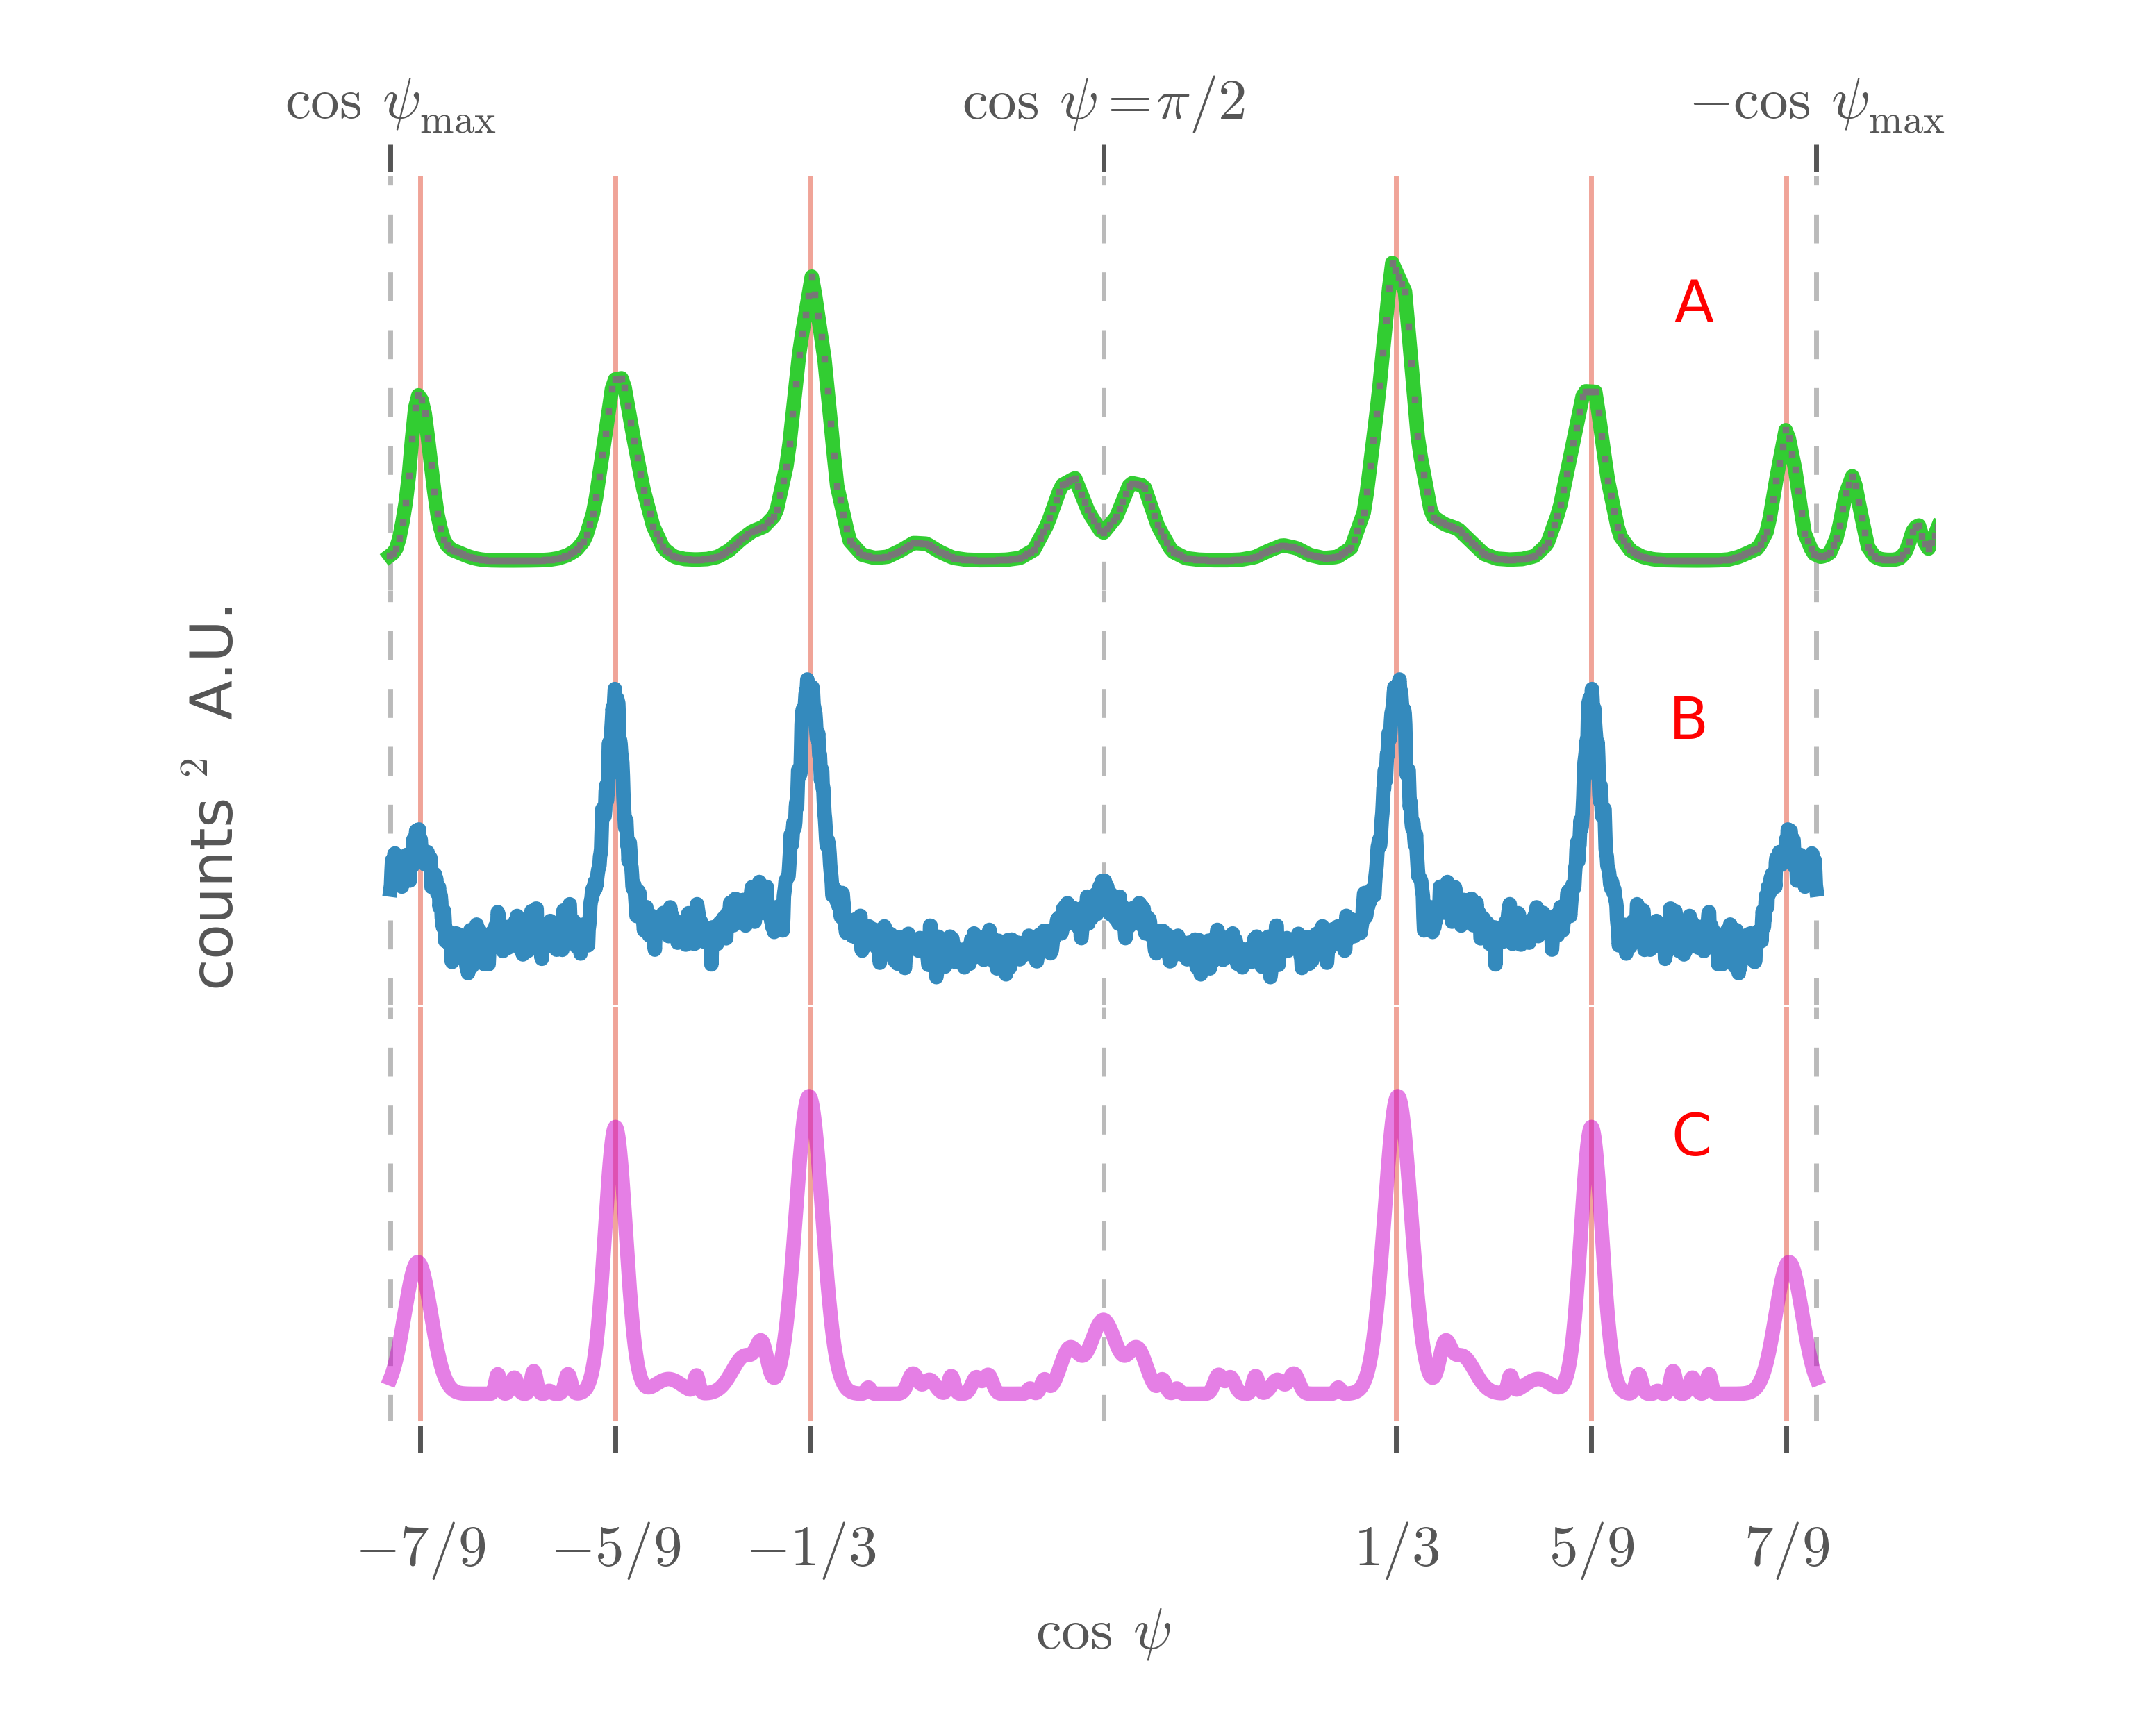
\includegraphics[scale=0.9]{./Fig4Mar8.png}
\caption{\emph{A} Simulated CXS for the gold decahedron in Figure \ref{fig:contrast}B. \emph{B} The mirror-symmetric difference correlation, $D_F(\cos \psi)$. \emph{C} The Gaussian fit $G(\cos \psi)$ (\S\ref{supp:Gauss}), fit directly to $D_F(\cos \psi)$.}
\label{fig:Main_result}
\end{figure}

After averaging (\ref{difcorz}) over $N=8\cdot 10^4$ exposures we were able to resolve clear CXS peaks at $\cos \psi = \pm\,  1/3, \pm\, 5/9, \pm\, 7/9$ indicating the presence of twinning (Figure \ref{fig:Main_result}). Figure \ref{fig:pk} shows signal-to-noise scaling for significant CXS peaks. As expected \cite{Kirian}, the signal to noise increases as the square root of the number of snapshots, $N$. A Z-score of $2.5$ is obtained after averaging $N=1000,\,1800,\,7200,$ and $\,85000$ snapshot exposures for peaks at $\cos \psi = \pm 1/3,\, \pm 5/9,\, \pm 7/9,$ and $0.4$, respectively. 
 
While the NNT model only predicts peaks at $\cos \psi = \pm1/3, \pm 5/9, \pm 7/9$, additional peaks with $Z > 2$ are also present (Figures \ref{fig:Main_result}, \ref{fig:pk}) that may indicate more complicated MTP structure. Each measured CXS peak represents a potential constraint on atomic models, and these additional peaks could be used to refine more complicated twinning patterns. The ability of CXS to identify complex atomic scale structures in ensembles of nanoparticles has potential for a wide range of applications. 
 
\begin{figure}[H]
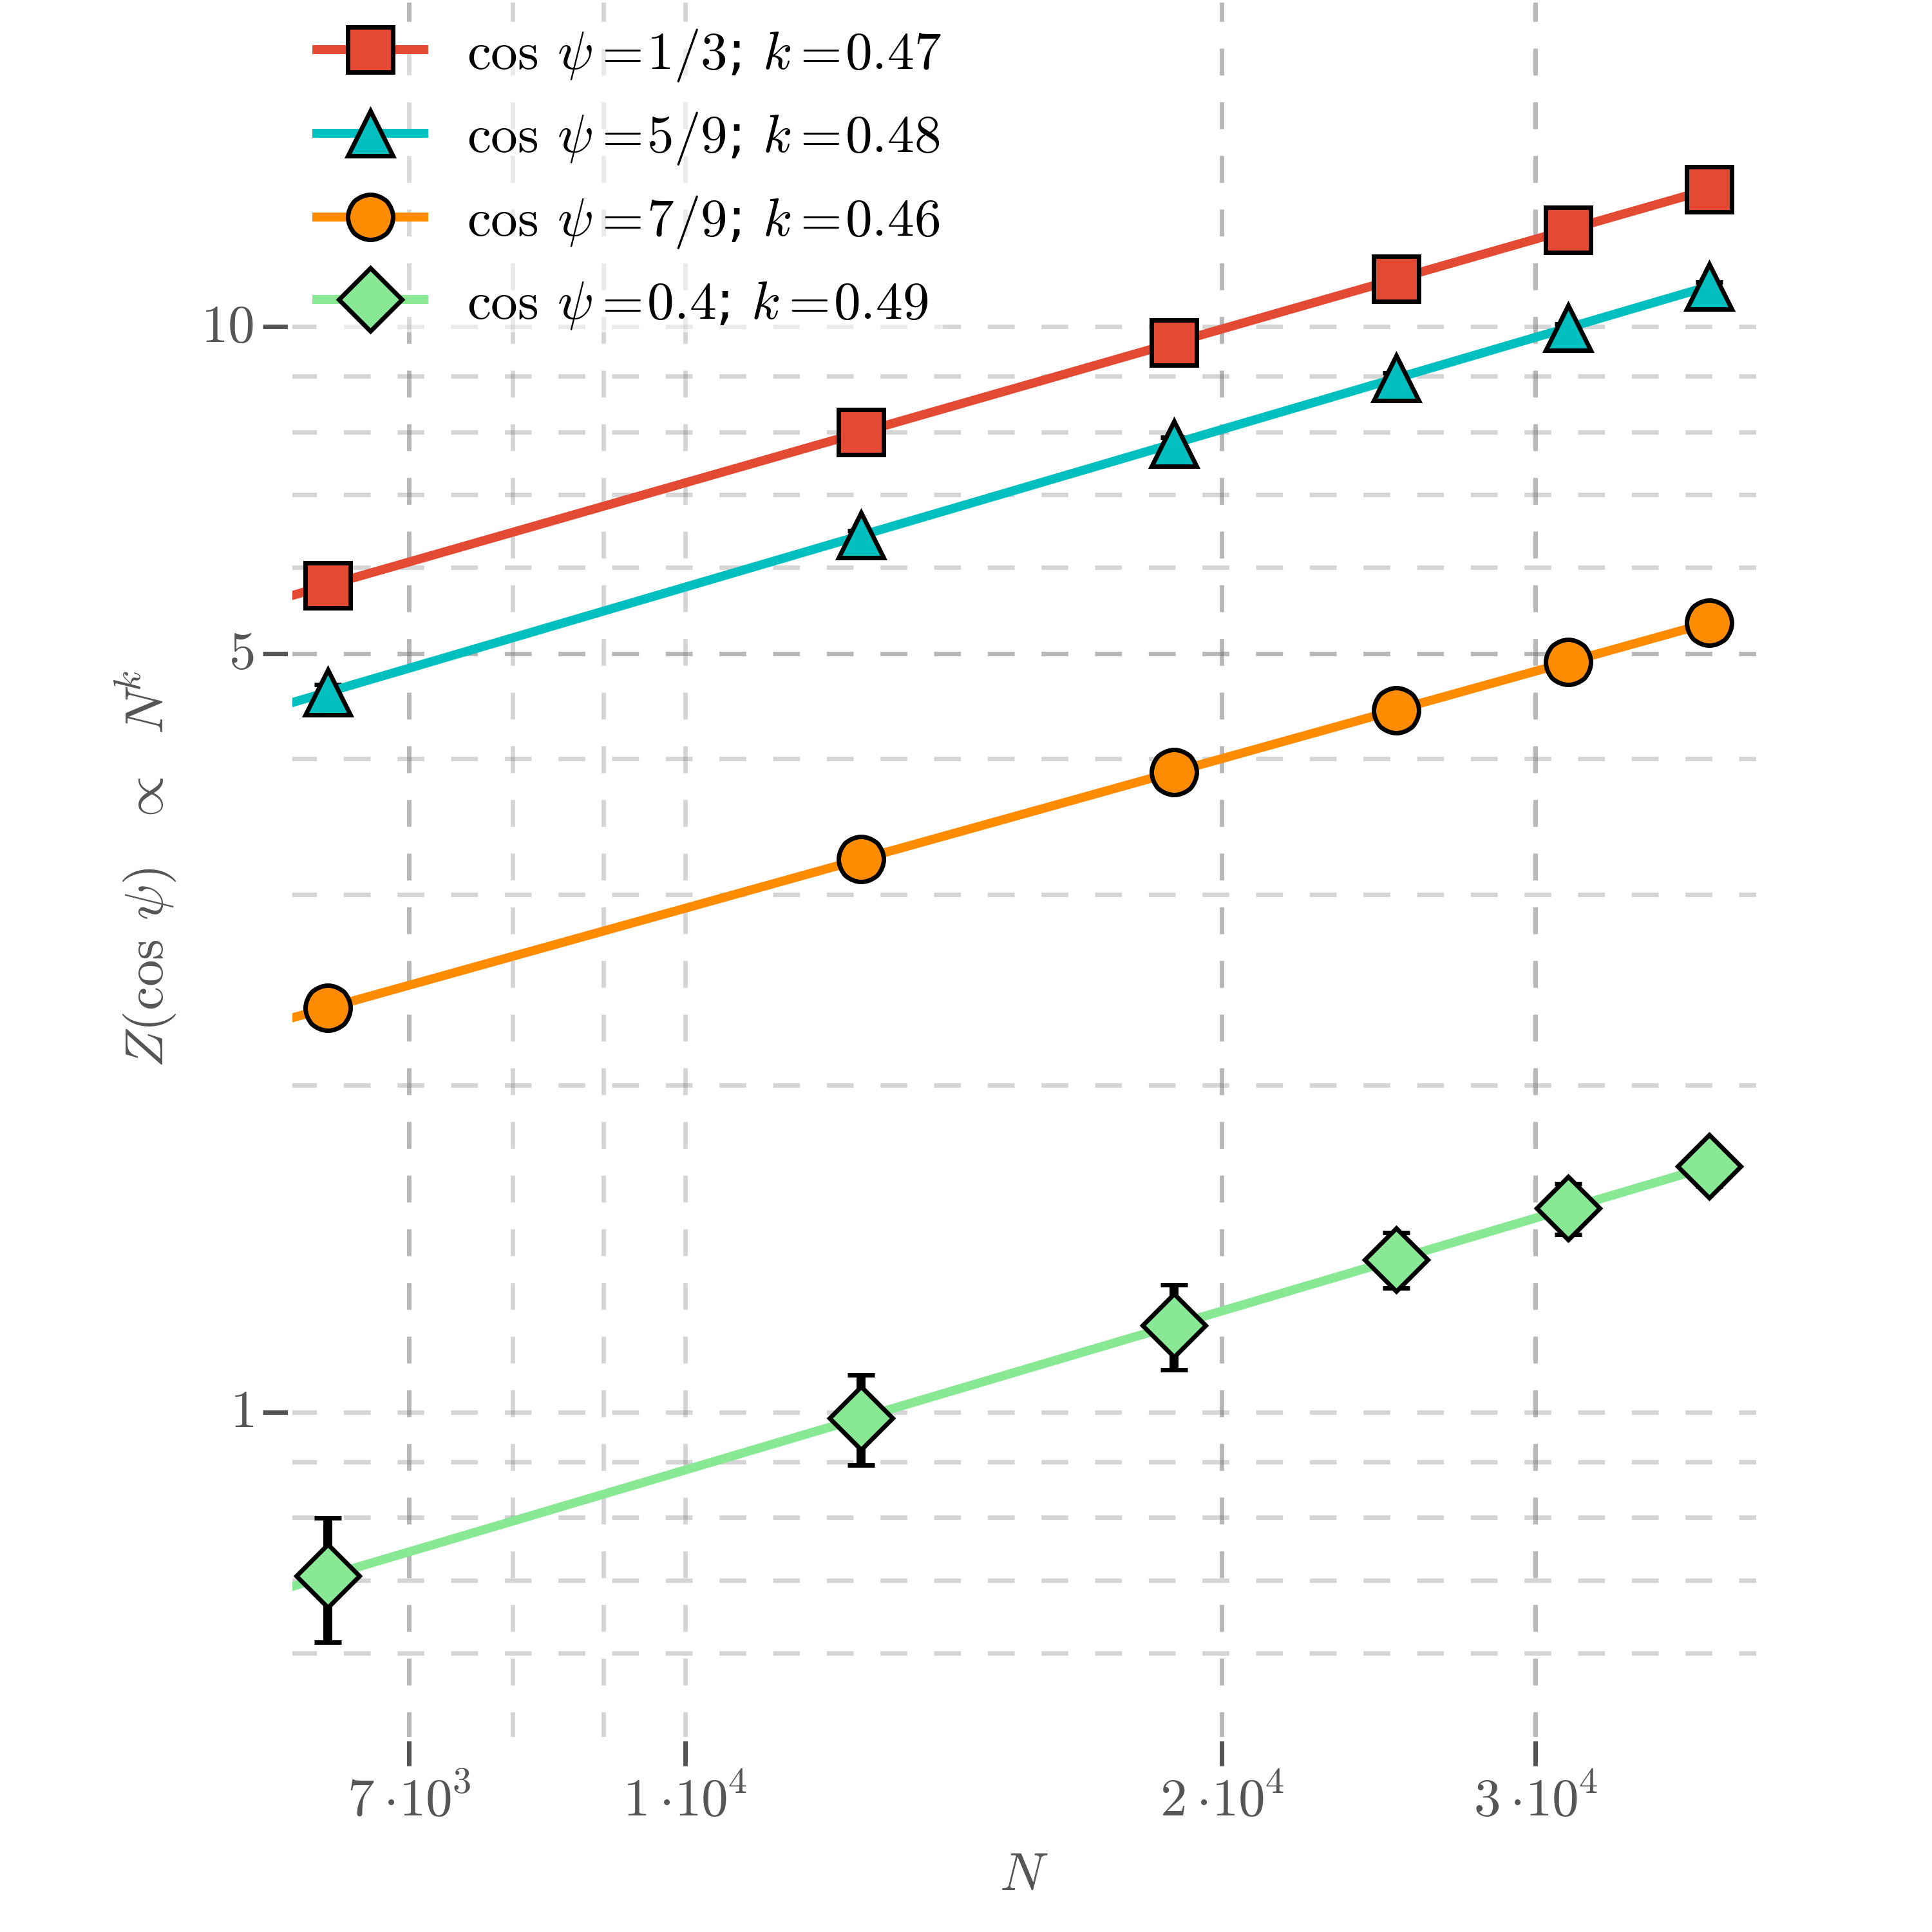
\includegraphics[scale=0.6]{./Fig5Mar8.png}
\caption{The estimated Z-score of 4 significant CXS peaks in $D(\cos \psi)$ as a function of $N$, the number of averaged exposure pairs. The Z-score is a measure of the signal to noise of the CXS peaks, and is defined in \S\ref{supp:Z}.}
\label{fig:pk}
\end{figure}
 
\section{Summary}
We have demonstrated the power of the CXS technique to obtain structural details of a large ensemble of similar objects at a resolution which can be used to compare with atomic models. From the statistics of observed features in the CXS we can assess the confidence level of the measured intensities of the different observed correlated scattering  features. Advances in X-ray instrumentation and sources have reached a critical point from which CXS has become feasible \cite{EmmaLaze, IshiLaze}. Consequently, the technique itself is in its infancy. The true power in a CXS measurement is in the richness of its information. Here we only reported on the measurement of intensity correlations at a single scattering vector, namely $q_{111}$ for gold FCC NPs, yet even more information is contained in the cross correlations and auto correlations of all measured scattering angles. As sample injection and data collection tools continue to improve, so should the ability to refine the angular intensity correlation functions hidden within snapshot X-ray measurements, providing a means for better model fitting and a better understanding of some of nature's smallest structures.

\section*{Acknowledgements}
The XFEL experiments were performed at the BL3 of SACLA with the approval of the Japan Synchrotron Radiation Research Institute (JASRI) (Proposal No. 2013B8009)
SD thanks  John Spence and Gordon J. Brown Jr for their advice and encouragement. Research supported by $\dots$. 

\begin{thebibliography}{9}

\bibitem{Kam77} 
Kam Z
\textit{Determination of macromolecular structure in solution by spatial correlation of scattering fluctuations.}
Macromolecules 10:927-934, 1977.

\bibitem{YacaShapeDepend}
Yacam\'{a}n MJ, Fuentes S, and Dominguez JM
\textit{The Effect of Shape and Crystal Structure of Small Particles on Their Catalytic Activity.}
Surf Sci, 106, 472-477 (1981)

\bibitem{ShapeDepend2}
Narayanan R and El-Sayed MA
\textit{Catalysis with Transition Metal Nanoparticles in Colloidal Solution: Nanoparticle Shape Dependence and Stability.}
J. Phys. Chem. B, 109, 12663-12676, 2005.

\bibitem{ShapeDepend3}
Narayanan R and El-Sayed MA
\textit{ Shape-Dependent Catalytic Activity of Platinum Nanoparticles in Colloidal Solution.}
Nano Lett., Vol. 4, No. 7, 2004

\bibitem{InoStability}
Ino S
\textit{Stability of Multiply-Twinned Particles.}
J Phys Soc Jpn, 941-953 (1969)

\bibitem{MarksWulff}
Marks LD 
\textit{Modified Wulff Constructions for Twinned Particles.} 
J. Cryst. Growth, 61, 556-566, 1983

\bibitem{MarksSurf}
Marks LD
\textit{Surface structure and energetics of multiply twinned particles}
Philos Mag A, 49, 81-93 (1984) 

\bibitem{KinTherm} 
Ringe E, Van Duyne RP, and Marks LD 
\textit{Kinetic and Thermodynamic Modified Wulff Constructions for Twinned Nanoparticles.}
J. Phys. Chem. C,  117, 15859��-15870, 2013

\bibitem{HeinemannStruct}
Heinemann K, Yacam\'{a}n MJ, Yang CY, and Poppa H
\textit{The Structure of Small, Vapor-Deposited Particles: I. Experimental Study of Single Crystals with Pentagonal Profiles.}
J of Cryst Growth, 47, 177-186 (1979)

\bibitem{YacaStruct}
Yacam\'{a}n MJ, Heinemann K, Yang CY, and Poppa H
\textit{The Structure of Small, Vapor-Deposited Particles: II. Experimental Study of Particles with Hexagonal Profile.}
J of Cryst Growth, 47, 187-195 (1979)

\bibitem{NPseeds} 
Langille MR et al
\textit{ Stepwise Evolution of Spherical Seeds into 20-Fold Twinned Icosahedra.}
Science 337, 954 (2012)

\bibitem{YangGeom} 
Yang CY 
\textit{Crystallography of decahedral and icosahedral particles: I. Geometry of twinning.}
Journal of Crystal Growth 47 274-282, 1979

\bibitem{YangSymm}
Yang CY, Yacam\'{a}n MJ,  and Heinemann K 
\textit{Crystallography of decahedral and icosahedral particles: II. High symmetry orientations.}
Journal of Crystal Growth 47 283-290, 1979

\bibitem{MarksGoldSilv}  
Marks LD and Smith DJ 
\textit{High-Resolution Studies of Small Particles of Gold and Silver 0.1. Multiply-Twinned Particles.}
J. Cryst. Growth 54, 425-432, 1981

\bibitem{YacaEM}
Yacam\'{a}n MJ and Borja MA
\textit{Electron Microscopy of Metallic Nano Particles Using High- and Medium-Resolution Techniques.}
Catal Rev Sci Eng, 34, 55-127 (1992) 

\bibitem{3Dimg} 
Chen CC et al
\textit{Three-dimensional imaging of dislocations in a nanoparticle at atomic resolution.}
Nature 496, 74-77, 2013

\bibitem{DaiShapes}
Dai ZR, Sun S, and Wang ZL
\textit{Shapes, multiple twins and surface structures of mono disperse FePt magnetic nanocrystals.}
Surf Sci, 505, 325-335 (2002)

%\bibitem{Friedel}
%Friedel G
%\textit{Sur les symetries cristallines que peut reveler la diffraction des rayons Rontgen.}
%Comptes Rendus hebdo-madaires de l'�Academie des Sciences 157:1533-1536, 1913

\bibitem{Kirian} 
Kirian RA, Schmidt KE, Wang X, Doak RB, and Spence JCH. 
\textit{Signal, noise, and resolution in correlated fluctuations from snapshot small-angle X-ray scattering.}
Phys. Rev. E 84, 011921, 2011

\bibitem{ImagingPotential} 
Neutze R, Wouts R, van der Spoel D, Weckert E, and Hajdu J 
\textit{Potential for biomolecular imaging with femtosecond X-ray pulses.}
Nature 406, 752-757, 2000

\bibitem{KamSynch} 
Kam Z, Koch MH, and Bordas J
\textit{Fluctuation X-ray scattering from biological particles in frozen solution by using synchrotron radiation.} 
Proc. Natl. Acad. Sci. USA 78, 3559-3562, 1981

\bibitem{MendezObserv} 
Mendez et al
\textit{Observation of correlated X-ray scattering at atomic resolution.}
Phil Trans R Soc B 369, 2014

\bibitem{SaldinBeyond}
Saldin et al
\textit{Beyond small-angle x-ray scattering: Exploiting angular correlations.}
Phys Rev B, 81, 174105 (2010)

\bibitem{SaldinIsolated}
Saldin DK, Shneerson VL, Fung R, and Ourmazd A
\textit{Structure of isolated biomolecules obtained from ultrashort x-ray pulses: exploiting the symmetry of random orientations.}
J Phys Condens Matter, 21, 134014 (2009)

\bibitem{SaldinTowards}
Saldin et al
\textit{Structure of a single particle from scattering by many particles randomly oriented about an axis: toward structure solution without crystallization?}
New J Phys, 12, 035014 (2010)

\bibitem{PandeDeduce}
Pande K, Schwander P, Schmidt M and Saldin DK
\textit{Deducing fast electron density changes in randomly orientated uncrystallized biomolecules in a pump - probe experiment.}
Philos Trans R Soc Lon Ser B, 369, 10130332 (2014)

\bibitem{Pedrini2D}
Pedrini B, Menzel A, Guizar-Sicairos M, Guzenko VA, Gorelick S, David C, Patterson BD, and Albela R
\textit{Two-dimensional structure from random multiparticle X-ray scattering images using cross-correlations.}
Nat Commun, 4, 1647 (2013)

\bibitem{Saldin2D}
Saldin DK, Poon HC, Bogan MJ, Marchesini S, Shapiro DA, Kirian RA, Weierstall U, and  Spence JCH
\textit{New Light on Disordered Ensembles: Ab Initio Structure Determination of One Particle from Scattering Fluctuations of Many Copies.}
Phys Rev Lett, 106, 115501 (2011)

\bibitem{StarodubSingle}
Starodub et al
\textit{Single-particle structure determination by correlations of snapshot X-ray diffraction patterns.}
Nat Commun, 3, 1276 (2012)

\bibitem{SaldinSingle}
Saldin DK, Poon HC, Schwander P, Uddin M, and  Schmidt M
\textit{Reconstructing an icosahedral virus from single-particle diffraction experiments.}
Opt Express, 19, 17318-17335 (2011)

\bibitem{KurtaMembrane}
Kurta et al
\textit{X-ray cross-correlation analysis of liquid crystal membranes in the vicinity
of the hexatic-smectic phase transition.}
Phys Rev E, 88, 044501 (2013)

\bibitem{SchroerFilms}
Schroer MA, Gutt C, and Gr\"{u}bel G
\textit{Characteristics of angular cross correlations studied by light scattering from two-dimensional microsphere films.}
Phys Rev E, 90, 012309 (2014)

\bibitem{Liu3D}
Liu H, Poon BK, Saldin DK, Spence JCH, and Zwart PH
\textit{Three-dimensional single-particle imaging using angular correlations from X-ray laser data.}
Acta Cryst A, 69, 365-373 (2013)

\bibitem{ChenDumbbell}
Chen G, Modestino MA, Poon BK, Schirotzek A, Marchesini S, Segalman RA, Hexemer A, and Zwart PH
\textit{Structure determination of Pt-coated Au dumbbells via fluctuation X-ray scattering.}
J Synchrotron Rad 19, 695-700 (2012)

\bibitem{ElserStrat}
Elser V
\textit{Strategies for processing diffraction data from randomly oriented particles.}
Ultramicrscopy, 111, 788-792 (2011)

\bibitem{SaldinTricks}
Poon HC and Saldin DK
\textit{Use of triple correlations for the sign determinations of expansion coefficients of symmetric approximations to the diffraction volumes of regular viruses.}
Struct Dyna, 2, 041716 (2015)

\bibitem{EmmaLaze}
Emma P et al
\textit{First lasing and operation of an angstrom-wavelength free-electron laser.}
Nat Photon, 4, 641-647 (2010)

\bibitem{IshiLaze}
Ishikawa T et al
\textit{A compact X-ray free-electron laser emitting in the sub-angstrom region.}
Nat Photon, 6 , 540-544 (2012)

\bibitem{Lehm2D}
Lehmk\"{u}hler F, Gr\"{u}bel G, and Gutt C
\textit{ Detecting orientational order in model systems by X-ray cross-correlation methods.}
J Appl Cryst, 47, 1315-1323 (2014)

\bibitem{GundDNA}
Schenk G, Krajina B, Spakowitz D, and Doniach S
\textit{Potential for measurement of the distribution of DNA folds in complex environments using Correlated X-ray Scattering.}
Mod Phys Lett B, 30 (2016)

\bibitem{HaiguangZern}
Liu H, Poon B, Janssen AJEM, and Zwart PH
\textit{Computation of fluctuation scattering profiles via three-dimensional Zernike polynomials.}
Acta Cryst A, 68, 561-567 (2012)

\bibitem{PandeTime}
Pande K, Schmidt M, Schwander P, and Saldin DK
\textit{Simulations on time-resolved structure determination of uncrystallized biomolecules in the presence of shot noise.}
Struct Dyna,  2, 024103 (2015)

\bibitem{Woch}
Wochner P et al
\textit{X-ray cross correlation analysis uncovers hidden local symmetries in disordered matter.}
Proc Natl Acad Sci USA, 106, 11511-11514 (2009)

\bibitem{Oxy}
Kurta RP, Chesnokov Y, Weckert E, and Vartanyants IA
\textit{Cross-correlation analysis of x-ray scattering from oxygen clusters.}
J Phys Conf Ser, 463, 012046 (2013)

\bibitem{AltarelliGen}
Altarelli M, Kurta RP, Vartanyants IA
\textit{X-ray cross-correlation analysis and local symmetries of disordered systems: General theory.}
Phys Rev B, 82, 104207 (2010)

\bibitem{Kurta2D}
Kurta RP, Altarelli M, Weckert E, and Vartanyants IA
\textit{X-ray cross-correlation analysis applied to disordered two-dimensional systems.}
Phys Rev B, 85, 184204 (2012)

\bibitem{MalmerbergOp}
Malmerberg E, Kerfield CA, and Zwart PH
\textit{Operational properties of fluctuation X-rat scattering data}
IUCrJ, 2, 309-316 (2015)

\bibitem{KamMicroG}
Kam Z
\textit{The reconstruction of structure from electron micrographs of randomly oriented particles.}
J Theor Biol 82, 15-39 (1980)

\bibitem{HowieMarks}
Howie A and Marks LD
\textit{Elastic strains and the energy balance for multiply twinned particles.}
Philos Mag A, 49, 95-109 (1984)

\bibitem{LCP1}
Ai X and Caffrey M
\textit{Membrane protein crystallization in lipidic mesophases: detergent effects.}
Biophys J, 79, 394-405 (2000)

\bibitem{LCP2}
Cheng A,  Hummel B,  Qiu H, and Caffrey M 
\textit{A simple mechanical mixer for small viscous lipid-containing samples.}
Chem Phys Lipids, 95, 11-21 (1998)

\bibitem{LCP3}
Caffrey M and Cherezov V 
\textit{Crystallizing membrane proteins using lipidic mesophases.}
Nat Protoc 4, 706-731 (2009)

\bibitem{LCP4}
Misquitta Y and M. Caffrey M 
\textit{Detergents destabilize the cubic phase of monoolein: implications for membrane protein crystallization.}
Biophys J, 85, 3084-3096 (2003) 

\end{thebibliography}


%%%%%%%%%%%
% SUPPLEMENTAL%
%%%%%%%%%%%
\newpage

\large{Supplemental Information: Wide-angle correlated X-ray scattering from gold nanoparticles demonstrated precise agreement with an atomic twinning model}

\setcounter{equation}{0}
\setcounter{figure}{0}
\setcounter{table}{0}
\setcounter{section}{0}
\setcounter{page}{1}
\makeatletter
\renewcommand{\theequation}{S\arabic{equation}}
\renewcommand{\thefigure}{S\arabic{figure}}
\renewcommand{\thesection}{S\arabic{section}}
%\renewcommand{\bibnumfmt}[1]{[S#1]}
%\renewcommand{\citenumfont}[1]{S#1}

\section{CXS simulation} \label{supp:sim}
We define a solution as a set of identical, non-interacting objects (e.g. molecules) $m$, each with an independent orientation $\bm \omega$ relative to the X-ray beam axis, governed by the objects diffusion constant. We consider $m$ as a collection of $N_a$ atoms each with position vector 
\be
\bm r^m_j (t) = \bm R^m_\omega (t)\cdot \bm r_j + \bm T^m(t) \qquad 1 \le j \le N_a
\ee 
where $\bm R^m_\omega(t)$ is a rotation operator, $\bm T^m (t)$ is a translation operator representing the center of mass position of $m$ at time $t$, and $\bm r_j$ is the position of the $j^{th}$ atom at an arbitrarily defined initial orientation. If we were to freeze the solution at an instant in time and expose it to X-ray photons of wavelength $\lambda$, then we could measure the scattering factor function

\be
S(\bm q, t) = \left | \sum_m^{N_m} \sum_{j}^{N_a} f_j(q) \,e ^ { -i \,\bm q \cdot \bm  r^m _j (t)  } \right |^2
\ee

Here $f_j(q)$ is the atomic form factor of the $j^{th}$ atom$, \bm q$ represents a position in reciprocal space (e.g. of a pixel) at scattering angle  

\be \label{angle}
\sin(\theta) = \frac{ \lambda }{ 4 \pi}\,q
\ee

and the outer sum is over all $N_m$ exposed objects. In general, $S(\bm q, t)$ may be written as

\be \label{ sums }
S( \bm q, t) = \sum_m^{N_m} \left | A^m_\omega (\bm q ,t ) \right|^2 + \sum _{ m \neq m' } A^m_\omega (\bm q,t ) \left (A^{m'}_\omega (\bm q,t ) \right )^*
\ee

where 

\be
A^m_\omega (\bm q,t ) = \sum_{j}^{N_a} f_j(q) e^{ -i \,\bm q \cdot \bm  r^m_j (t)  }
\ee

The strength of the interference term on the RHS of (\ref{ sums }) depends on both the concentration of the sample and the magnitude of the scattering angle (\ref{angle}). For larger angles and more dilute samples, the factors $e^{-i \bm q \cdot (  \bm T^m - \bm T^{m'})}$ will approach zero, and we can safely neglect this term such that we have

\beq \label{ scatter}
S( \bm q, t) &=& \sum_m^{N_m} \left | A^m_\omega (\bm q,t ) \right|^2 \\
&=& \sum_m^{N_m} \left | \sum_{j}^{N_a} f_j(q)\, e^ { -i \,\bm q \cdot \bm  r^m _j (t)} \right | ^2   \\
&=& \sum_m^{N_m} \left | \sum_{j}^{N_a} f_j(q)\, e^ { -i \,\bm q \cdot \left (\bm {R}^m_\omega \left(t\right)\cdot \bm r_j \,+\, \bm {T}^m\left(t\right) \right)} \right | ^2 \\
&=& \sum_m^{N_m} \left | \sum_{j}^{N_a} f_j(q)\, e^ { -i \,\bm q \cdot \bm {R}^m_\omega (t)\cdot \bm r_j }  \right | ^2 
\eeq

Therefore the measured scattering factor for a "dilute" solution is simply a superposition of single molecule scattering factors at various orientations $\bm \omega$.  Instead of considering the precise time dependence of each object (molecule) in solution, however, we consider that on average each orientation $\bm \omega$ is occupied by a fixed number of molecules $N_\omega = (N_m/ \int d\omega)$, and that at each instant, this number is fluctuating by some small amount $\alpha( \bm \omega, t )$ (we are borrowing notation directly from \cite{Kam77}). Consider the average isotropic scattering factor over total molecules

\be
S(q) = N _\omega \int S( \bm q, \bm \omega ) d\omega 
\ee

where 

\be \label{scattering}
 S(\bm  q, \bm \omega )  = \left | \sum_{j}^{N_a} f_j(q)\, e^ { -i \,\bm q \cdot \bm {R}_\omega \cdot \bm r_j } \right | ^2 
\ee

is the scattering factor of a molecule at orientation $\bm \omega$. Then we can represent $S(\bm q, t)$ as 

\be
S(\bm q, t )  = S ( q )  + \int  S( \bm q, \bm \omega ) \alpha( \bm \omega ,t) d\omega 
\ee

Zvi Kam's main statement is that by measuring 

\be 
\left \langle S(\bm q_1, t )  S(\bm q_2, t )   \right \rangle_t - S( q_1 ) S( q_2 )
\ee

one would resolve a correlation function 

\be
C( \bm q_1, \bm q_2  ) = N_\omega \int S( \bm q_1, \bm \omega ) S( \bm q_2, \bm \omega ) d\omega
\ee

\be \label {kamzcor}
C( q_1, q_2, \cos \psi   ) \propto \int S( \bm q_1, \bm \omega ) S( \bm q_2, \bm \omega ) d\omega
\ee

which depends only on the single particle scattering factor.  The scattering factor equation (\ref{scattering}) is what we simulate, given an arrangement of atoms. We can then easily calculate the expected CXS signal by evaluating the integral (\ref{kamzcor}). 


\section{Data fitting and Friedel symmetry constraint}
\subsection{Gaussian fitting} \label{supp:Gauss}

First, after averaging all snapshot difference correlations, we determined a set $\Gamma$ of local maxima $\cos \psi_\gamma$ in $D_F(\cos \psi)$. Peaks were determined by applying a Savitzky-Golay filter and a smoothing convolution to $D_F(\cos \psi)$, shown here

\begin{figure}[H]

\end{figure}[H]

Then for each $\cos \psi_\gamma \in \Gamma$ we defined a Gaussian function

\be
G_\gamma (\cos \psi \,;\,  d, \, A)  =  d +  A\,\exp \left [ \frac{-\left( \cos \psi - \cos\psi_\gamma \right)^2}  {2\,\eta^2}  \right ]
\ee 

with constrained width, $\eta$, and mean, $\cos \psi_\gamma$. The offset $d$ takes into account any residual background terms and the amplitude $A$ is our measure of CXS signal from the gold NPs.

By employing non-linear least squares we obtained the fits $(d_\gamma, A_\gamma)$ to each detected peak. With these fits, the total fitted CXS signal can be represented by a sum of Gaussians

\be \label{fit}
G(\cos \psi) = \sum_\gamma \,\,G_\gamma ( \cos \psi \,;\, d_\gamma, A_\gamma) - d_\gamma
\ee

Practically, we fit partial sums and optimized the parameters in parallel. 
\subsection{Friedel symmetry constraint} \label{supp:Fried}
Each measured CXS peak represents a potential constraint on atomic models. Successful model fitting will depend on one's ability to distinguish physical CXS peaks from artifactual CXS peaks. To this end we can employ a Friedel symmetry constraint. Friedel symmetry states that $I(\bm q) = I(-\bm q)$ (in the absence of anomalous scattering). Hence, if one measures a correlation at angle $\psi = \arccos ( \bm q_1 \cdot \bm q_2)$, one should measure the same correlation at angle $\pi - \psi = \arccos( -\bm q_1 \cdot \bm q_2)$. This implies that a CXS function should be mirror-symmetric about $\psi = \frac{\pi}{2}$ ($\,\cos \psi=0$). Any signal violating this symmetry is likely artifactual. 

We define the Friedel difference correlation 

\be
D_F(\cos \psi) = \frac{D(\cos \psi)  +\, D(-\cos \psi)}{2} 
\ee

which enhances true CXS information while minimizing artifactual asymmetric correlation peaks.

\section{Scaling of the signal with the number of snapshots} \label{supp:Z}

\subsection{Definition of the Z-score} 
We define the Z-score of the Gaussian fit amplitudes $A_\gamma$ in (\ref{fit}) to be

\be
Z_\gamma = \frac {A_\gamma  - \mu }{\sigma}
\ee

where $\mu \rightarrow 0$ for difference correlations, and  $\sigma$ is estimated to be the standard deviation of the inter-difference correlation, defined as  

\be \label{ucorz}
D_{i,j,k,l}(\Delta) =\big \langle  \,\big(  I_i(\phi)-I_j(\phi) \big)\,\big( I_k( \phi + \Delta) - I_l( \phi+\Delta) \big) \big \rangle _{\phi}
\ee

We compute (\ref{ucorz}) by randomly selecting pairs $i,j$ and $k,l$ from $\mathcal P$. If the snapshots were paired in a way that minimizes artifactual variations, then the variance of (\ref{ucorz}) is a good estimate of the theoretical noise $\sigma$ associated in a CXS measurement. This technique for noise estimation is useful in situations where CXS signal is continuous, e.g. in the case of soft matter and smaller NPs with broad Bragg reflections.

\subsection{Bootstrap statistics on the Z-score}

We assume there is a total of $N$ snapshot exposures grouped into $N_\mathcal{P}$ pairs. The two finite Z-score parameters $A_\gamma$ and $\sigma$ are both functions of $N_\mathcal{P}$. Therefore we can randomly sample $N_\mathcal{P}$ pairs from $\mathcal P$, compute the Z-score, and repeat for a total of 200 times. The plotted Z-score is then the mean of these samplings, and the error bar represents one standard deviation of these samplings.

\section{Data analysis stream}
\begin{figure} [H]
\includegraphics[]{ana_flow_chart_2.png}
\label{fig:flow}
\caption{A schematic showing the flow of data, from the raw data, to the final CXS signal. It is a bit complicated, and we will outline some of the key processes (black boxes) in this supplemental material}
\end{figure}

We would like to calculate the correlated X-ray scattering (CXS) for gold nanoparticles

\begin{equation} \label{supp:c111}
C(\Delta) = \sum_i^N  \left \langle \,I_i( \phi) \,I_i(\phi +\Delta) \right \rangle _\phi
\end{equation}

for all $\phi$ on $[0,2\pi]$, where $I_i(\phi)$ is the scattering intensity from exposure $i$, measured along a Bragg ring at $q_{111}=(4\pi/\lambda)\,\sin(\theta_{111})$.

\subsection{Convert data}
Scattered photons were recorded on an area detector perpendicular to the forward photon beam. The detector we used was the MPCCD octal sensor, consisting of 8 application-specific integrated circuits (ASICs) which are read out simultaneously, up to 60 Hz. The raw data 

\begin{itemize}
\item are stored on an external user-restricted server, where they remain for one year before being moved to tape storage. 
\item are accessed using in-house SACLA data conversion programs, which output the data as user-accessible hdf5 files.  
\end{itemize}

The in-house software has an option to store reconstructed images, which we employ. The ASICs are assembled into an approximate image, and the relative gains are adjusted. 

The reconstructed MPCCD images each have $2399\times 2399$ pixels. The boundary of the image is padded with zeros (Figure \ref{supp:cart2pol}), so that the reconstructed image size doesn't change if the panels themselves are adjusted between experiments. Each pixel has an integer coordinate $(\,p_x, p_y)$, which also serves as it's array index. We denote the measurement of each pixel during an exposure $s$ as $I_i^{ \mathrm{cart} }(\,p_x\,, \,p_y)$ where ``$\text{cart}$" indicates the image is in cartesian coordinates.


\subsection{Polar interpolation}
Our first task is performing a polar interpolation on the data

\be
I_i^{ \mathrm{cart} }(\,p_x\,, \, p_y) \rightarrow I_i(\,p_r\equiv r \,, p_\phi \equiv \phi)
\ee

for a narrow range of $r \,\in\, [\,r_{\text{low}}\,,\, r_{\text{high}}\,]$ which encompasses the Bragg ring $q_{111}$ (Figure \ref{supp:cart2pol}). This serves to reduce the effective size of the data, which is good for an analysis stream on a large dataset. Loading hundreds of thousands of large images in and out of random-access memory can slow down computation significantly. In this sense it is better to work with a snippet of each image that we find interesting, which in this case is the region near Bragg ring.

The azimuthal pixel value, 

\be
\phi = \arctan\left( \frac{p_y - p_b}{p_x - p_a} \right )
\ee

where  $(\,p_a\,,p_b)$ is the point where the X-ray beam axis intersects the detector. This is the same  as the reciprocal space angle $\phi$ in (\ref{supp:c111}). We approximate that $(\,p_a\,,p_b)$ remains constant throughout the experiment. One can extrapolate this point of intersection by using the Bragg rings themselves under the assumptions that they are circularly symmetric about the beam axis, and that the detector is perpendicular to the beam axis.

The radial pixel value $r$ is related to the scattering angle $q$ via

\be
r = \frac{d}{\Delta p}\,\,\tan\left(2\,\arcsin \left( \frac{q\,\lambda}{4\,\pi}  \right) \right)
\ee

, where $d$, $\Delta p$, and $\lambda$ are the sample-to-detector distance, square pixel length, and photon wavelength, respectively.

With these definitions, we use an elementary floor-nearest-neighbor approximation to approximate the polar image:

\begin{equation} \label{polimg}
I_i(r \,, \phi) = I_i ^{ \mathrm{cart} }\left ( \lfloor\,  r \,\cos(\phi)+p_a \rfloor, \lfloor\, r\, \sin(\phi) +p_b \rfloor \right)
\end{equation}

where $\lfloor\,\rfloor$ is the floor operation.

\begin{figure}[H]
\includegraphics[]{supp_figs/CART_TO_POLAR.pdf}
\caption{A reconstructed image, and the result of a floor-nearest-neighbor interpolation across the $q_{111}$ Bragg ring. The polar image shown has the same resolution as the cartesian image.}
\label{supp:cart2pol}
\end{figure}

\subsection{Working with a mask}
In all of our analysis, we work with masked images. We let $M(r\,,\phi)$ represent the polar image mask, a binary image used to exclude the gaps and boundaries surrounding the ASICS in the reconstructed images. Masked pixel values are $0$ and usable pixel values are $1$. Typically there is a mask $M^{\text{cart}}$ for the cartesian images. In this case we would define the polar mask to be $$M(\,r\,, \phi) = M^{\text{cart}} \left ( \lfloor\, r\,\cos(\phi)+p_a \rfloor, \lfloor\,r\, \sin(\phi) +p_b \rfloor \right)$$
Commonly, large scale sensors like these have signal spikes near the edges, so the ASIC edges should be included in the mask. As an example, the mean signal in a masked polar image is defined as

\begin{equation} \label{average_signal}
\bar I_i =  \frac
{\left(\sum\limits_{r\,,\,\phi}\, M( r\,,\phi )\,\,I_i(r\,,\phi) \right) }
 {\left (\sum\limits_{r\,,\,\phi}\, M ( r\,,\phi )\right )}
\end{equation}

For our experiment, we used a fixed mask $M^{\text{cart}}$ and hence $M$ for all images, but these can also vary throughout a given experiment.

%\subsection{Parameterizing the images}
%It is useful in later stages of the analysis to have certain measures for each image. We can use these measures for clustering the data, pairing exposures (which is critical in our analysis, and will be discussed below) and filtering out the images that appear to be corrupted or lacking signal.
%
%From each polar image \ref{polimg} we record several values. These values include obvious measures, such as the mean signal. In addition, however, we would like to store some specialized quantities described below.

\subsection{The 111 Bragg ring position}

\begin{figure}[H]
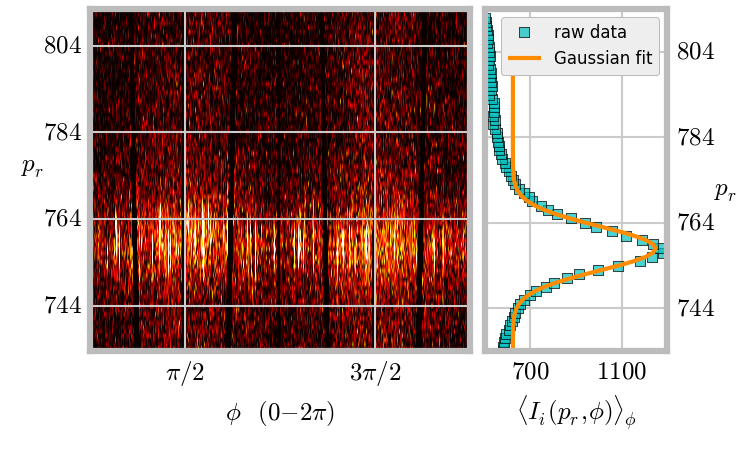
\includegraphics{supp_figs/bragg_ring_position.png}

\caption{Left) A polar image $I_i(r, \phi)$ representing a single snapshot of the gold nanoparticles. Right) The azimuthally averaged intensity and a corresponding Gaussian fit. The center of the Gaussian corresponds to the $\{111\}$ Bragg ring radial position, $r^*_i$}
\end{figure}
In this particular experiment the sample jet was unstable. Consequently, the sample-to-detector distance fluctuated on a shot by shot basis. In extreme cases, the viscous lipid-cubic-phase solution would kink and clog around the syringe needle tip, causing significant fluctuations in $r^*$ (Figure \ref{supp:p111}).

We will denote the $\{111\}$ Bragg ring radial position snapshot exposure $i$ by $r^*_i$, i.e. the radial pixel ring corresponding to $q_{111}$. Since we do not know the precise sample-to-detector distance of each exposure $s$, we estimate 

\be
r^*_i   \,=\, \text{argmax} \left[ \big \langle I_i \left(\,r\,, \phi\right)\, \big \rangle_{\phi} \right]
\ee

where $\langle \dots \rangle _{\phi}$ denotes the discrete average over $\phi$. Therefore, $r^*_i$ is maximum $r$ across the radial profile of the polar image. Because gold is the only sample component which scatters at these high angles, we assume this is a robust approach.

\begin{figure}[H]
\caption{A histogram of the radial pixel ring corresponding to  $q_{111}$. We predict that the shape of this histogram with the two peaks near 760 and 772 represent arises due to fluctuations in the injector system leading to different sample-to-detector positions. One way to fix this would be to use a gas focuses sample injector. We analyzed exposures bound by the orange lines.}
\includegraphics[]{supp_figs/Fig_p111_supp.pdf}
\label{supp:p111}
\end{figure}

\subsection{The Bragg ring (angular profile) $I_i(\phi)$}
For  the purpose of this paper, we found it sufficient to let 
\be
I_i(\phi) = I_i(r=r^*_i, \phi)
\ee
%While more sophisticated techniques exists, here we simply average radially across a %small portion $\delta r^*$ of the Bragg ring at each $\phi$:
%\begin{equation}
%I_i(\phi) = \big \langle I_i \left(\,r\,, \phi\right) \big \rangle _{r \,\in\, \delta r }
%\end{equation}
%where $\langle \dots \rangle_{r}$ is a discrete average over $r$ on the interval 
%$$\delta r = \big [\, r^*_i - \delta r^* \, \,,\,\, r^*_i + \delta r^*\, \big ]$$
%The value $\delta r^*$ is usually a few pixels.
We sample $\phi$ at $N_{\phi}$ evenly spaced points along the Bragg ring. We fix $N_\phi \ge 2\,\pi\,p_{\text{high}}$. In this way we will sample azimuthally at unit pixel precision at the highest anticipated angles. We let $\varPhi_i$ be the set of all non-masked sampled $\phi$ values in shot $i$:
\be \label{setphi}
\varPhi_i = \left \{ \phi \in   \left \{0\,, \frac{2\,\pi}{N_\phi}\,, \frac{4\,\pi}{N_\phi}\,, \dots \frac{2\,\pi\,(N_\phi-1)}{N_\phi} \right \}\, \big | \,\,M_i(\phi) = 1\right  \}
\ee
where
\be
M_i(\phi) = \left \lfloor \,\, M \left( \,r=r^*_i \, , \phi \right )  \right \rfloor
\ee
is the corresponding polar mask, floored because it is binary.
\begin{figure}[H]
\includegraphics[]{supp_figs/Fig_angprof_supp.pdf}
\caption{In blue is the raw calculation of $I_i(\phi)$ for a single snapshot, which shows sharp peaks indicative of larger crystallites. Our motivation is actually to study less crystalline materials in the soft matter regime, so we attempt to remove all signal associated with these larger, more crystalline nanoparticles. The solid yellow line is a biased polynomial, fit to the raw data with the signal spikes (blue x markers). Shown in dashed-black is the unbiased polynomial $y*_i(\phi)$, fit to the data without the Bragg peaks (red triangle markers).}
\label{supp:prof}
\end{figure}

\subsection{Quantifying angular anisotropies}

As one can see in (Figure \ref{supp:prof}), there is a large, slow-varying angular anisotropy in the angular profile of the Bragg ring $I_i(\phi)$. We seek to suppress any errors this will introduce into the correlation function (\ref{supp:c111}). 

Shadows, beam polarization, and sample inhomogeneity, are a but a few sources of systematic noise which can give rise to large angular anisotropies in $I_i(\phi)$. One can see these by eye (Figures \ref{supp:cart2pol}, \ref{supp:prof}). When correlated via (\ref{supp:c111}), these will dominate the tiny CXS signals due to the gold nanoparticles. We have a method for overcoming these effects, which depends on the pairing of exposures with similar anisotropies. Here we discuss the quantification of the angular anisotropy.

In order to quantify the anisotropy, we fit 15th degree Chebyshev polynomials of the first kind to the angular intensity profile $I_i(\phi)$. Chebyshev polynomials of the first kind are defined by

\begin{equation}
y(\phi) = c_0\,T_0(\phi) + c_1\,T_1(\phi) + \dots + c_{15} \, T_{15}(\phi) 
\end{equation} 

where 

\begin{eqnarray}
T_0(\phi) &=& 1 \nonumber\cr
T_1(\phi) &=& x \nonumber \cr
T_{n+1}(\phi) &=& 2\,x\,T_n(\phi) - T_{n-1}(\phi) \nonumber
\end{eqnarray}

The fit is a simple least squares which minimizes the residual

\begin{equation} \label{supp:fit}
E =  \sum_{\phi} \big |\, f(\phi) - y(\phi)\big |^{\,2}
\end{equation}

Note in (Figure\ref{supp:prof}) the large Bragg spots (peaks). These large signal spikes will bias the residual $E$, hence we mask them prior to fitting the polynomial. To detect the signal spikes we use the median outlier filter described in \S $\ref{outlier_filter}$. We let $y^*_i$ be the Chebyshev polynomial which minimizes the un-biased residual. Figure \ref{supp:prof} shows two polynomial fits, one to the raw data and another to the data without the Bragg spots. The pairing of exposures according to their angular anisotropies is critical for our analysis, as detailed in the following sections.

\subsection{Exposure pairing}
For our reported results, we made use of the difference correlation, which involves subtracting pairs of exposures, and correlating the residuals. Our data were divided up into $85$ experimental  runs $\mathcal R$, and each run represents an average of $4500$ usable exposures. We considered a usable exposure to be one where the X-ray shutter was open, and the X-ray laser was operating properly (occasionally the laser pulses would cease during a run from complications upstream). We acquired roughly $3.8 \cdot 10^5$ usable exposures, and we did not attempt to compare each exposure with every other exposure. Rather, we only compared and paired exposures that occurred during the same experimental run.

\begin{figure}[H]
\includegraphics[]{supp_figs/shot_mean_histogram.pdf}
\caption{A histogram of the mean intensity of every polar image $I_i(r,\phi)$ across all experimental runs. Only exposures whose mean intensity was greater than 300 units and less than 3000 units were analyzed $(300 \le \bar I_i \le 3000)$.}
\label{fig:shot_mean_histogram}
\end{figure}
%We call the set of all exposures $\{i\}$, and the set of exposures per run $\{i\}_{\mathcal R}$.  
We began by selecting all exposures for analysis according to their total average signal $\bar I_i$ as defined in (\ref{average_signal}) (Figure \ref{fig:shot_mean_histogram}). We ignored exposures that were too weak $(\bar I_i < 300 \mathrm{\,counts})$ because it is likely that they were recorded when the sample injector failed. Similarly, we rejected exposures that were too strong $(\bar I_i > 3000 \mathrm{\,counts})$ for they may include non-liner effects on the detector such as faulty pixel responses.

After filtering based on mean intensity, exposures within a certain run were grouped according to their respective $r^*_i$. Each exposure $i$ was assigned to a subgroup based on the floored value $\lfloor r^*_i \rfloor$, i.e. the closest integer less than $r^*_i$ (the vertical orange lines in (Figure \ref{supp:p111}) represent the group bins). Pairs were constrained to be formed using exposures from the same subgroup. The pairing process involved an optimization step in which exposures were recursively compared to each other; forming subgroups for pairing serves to reduce the required computation time. 

\emph{We required that an exposure can only be used once during analysis}. Each  exposure $i$ was paired with an exposure $j$ according to their azimuthal anisotropies, quantified by the fitted polynomials $y^*_i,\, y^*_j$  (azimuthal anisotropies should be similar for similar positions $r$ on the polar image; the subgrouping described above is advantageous in this regard). We used the squared Euclidian distance

\be
\epsilon_{i,j} = \sum\limits_\phi  \left ( y^*_i (\phi) -  y^*_j (\phi) \right ) ^2
\ee

as a metric of comparison between two exposures. Let $\mathcal P$ represent a set of pairings, in which each exposure is paired, and no exposure is paired twice (it is understood that if their is an odd number of exposures in a subgroup, then a single shot will remain unpaired and thus not used in the analysis). We can define the total distance between paired exposures as

\be
d = \sum_{i,j \in \mathcal P} \epsilon_{i,j}
\ee

A good pairing seeks to minimize $d$. This is a computationally hard problem, however, so we approximate it.

\subsection{Compute Differences}
The angular difference profile is defined as

\begin{equation}
D_{i,j}(\phi) = I_i(\phi) -I_{j}(\phi) 
\end{equation}

We combine the angular profile masks (which mask detector, large Bragg spots, etc) as

\begin{equation}
M_{i,j}(\phi) \,\,= \,\,M_i(\phi)\,\,M_j(\phi)
\end{equation}

We then normalize each difference profile according to the mean signal

\be
\bar D_{i,j} = \frac{ \sum_\phi M_{i,j}(\phi) \, D_{i,j}(\phi)  } {\sum_\phi M_{i,j}(\phi)}
\ee

We define the normalized difference intensity as

\be
\hat D_{i,j}(\phi) = D_{i,j}(\phi) / \bar D_{i,j}
\ee

\subsection{Correlate}

Now we discuss the actual correlation computation. Typically it should be straightforward but we are correlating masked functions, and proper handling of the mask is essential. For each angle $\Delta$ where we compute the correlation, we must keep track of the number of non-masked $\phi$ pairs, e.g. 

\begin{equation}
N_{\Delta\,,\,M} = \sum\limits_{\phi} M_{111}^{\,s\,,\,s_{\min}}(\phi)\,\,M_{111}^{\,s\,,\,s_{\min}}(\phi + \Delta)
\end{equation}

The difference correlation for exposures $s,s_{\min}$ is then given by 


\begin{equation}
\tilde c_{111}^{\,s\,,\,s_{\min}}(\Delta) = 
\frac
{1}
{N_{\Delta\,,\,M}}
\sum\limits_{\phi}
\bigg( \hat D_M^{\,s,\, s_{\min}}(\phi)\bigg)
\bigg(\hat D_M^{\,s,\, s_{\min}}(\phi + \Delta) \bigg)
\end{equation}

where we define

\begin{equation}
\hat D_M^{\,s,\, s_{\min}}(\phi) \equiv \hat D_{111}^{\,s\,,\,s_{\min}}(\phi)\,M_{111}^{\,s\,,\,s_{\min}}(\phi)
\end{equation}

This operation is slow. We can make use of the convolution theorem, however, and compute the operation

\begin{equation} \nonumber
\mathbb G_\Delta = 
\mathbb F_\Delta^{-1} 
\bigg[  
\mathbb F_\Delta\big[ \hat D_M^{\,s,\, s_{\min}}(\phi)  \big]\, 
\left( \mathbb F_\Delta\big[\hat D_M^{\,s,\, s_{\min}}(\phi) \big]\right)^{\,\*}
\bigg]
\end{equation}

where $\mathbb F_\Delta, \mathbb F_\Delta ^{-1}$ are the real-valued Fourier transform, and real-valued inverse Fourier transform operations, respectively. By the convolution theorem we have 

\begin{equation}
\tilde c_{111}^{\,s\,,\,s_{\min}}(\Delta) = \mathbb G_\Delta 
\end{equation}

therefore, by making use of the fast Fourier transform algorithm, one can speed up the computation (14).

Usually, one would need to be employ costly techniques to evaluate $\mathbb F$ on the non-uniform, masked domain, however, because the average value of a difference ring profile is $0$, one can compute $\mathbb F$ on the full uniform domain for $\phi$, i.e. for 

\begin{equation}
\phi \in \left \{ 0\,, \frac{2\,\pi}{N_\phi}\,, \frac{4\,\pi}{N_\phi}\,, \dots \frac{2\,\pi\,(N_\phi-1)}{N_\phi} \right \}
\end{equation}
Therefore, the only additional computation involving the mask is the evaluation of the product (15).

\subsection{Filter all difference correlations and average}

At this stage we have computed (14) for each $(s,s_{\min}) \in \mathcal P_{r}$ and for all runs $r \in \mathcal R$ where $r$ is a run label and $\mathcal R$ is the set of all run labels. We define 

\begin{equation}
\mathcal P^{\,N_{\text{pairs}} } = \underset{r\,\in\,\mathcal R}{\cup} P_r
\end{equation}

where $N_{\text{pairs}}$ is the total number of filtered exposure pairs. We define 

\begin{equation}
\mathcal P^{N} \subset \mathcal P^{\,N_{\text{pairs}}}
\end{equation}

where $N \le N_{\text{pairs}}$ is the cardinality of $\mathcal P^N$. With this, we define the CXS signal as a function of N

\begin{equation}
\tilde C_{111}(\Delta) = 
\big \langle \tilde c_{111}^{\,s\,,\,s_{\min}}(\Delta) \big \rangle
_{(s\,,\,s_{\min})\,\in\,\mathcal P^N} 
\end{equation}

\section{Median absolute deviation filter steps} \label{outlier_filter}

Given an observation $f(x)$, e.g. an angular intensity, 

\begin{itemize} 
\item Find the standard deviation from the median of each observation $f(x)$, i.e. 
\be
\sigma(x) = \sqrt{ \left ( f(x) - \text{median} \left [\,f(x) \,\right ] \right) ^{\,2}}
\ee
\item Set the modified Z-score for each observation to be 
\be
z(x) = 0.6745 \,\, \left( \frac{\sigma(x)}{\text{median}\left[\,\sigma(x)\,\right]} \right )
\ee

\item Check whether $z(x)$ is greater than some outlier threshold. Outliers will have $z(x)$ greater than the threshold.
\end{itemize}
  

\begin{thebibliography}{9}
\bibitem{Kam77} 
Kam Z
\textit{Determination of macromolecular structure in solution by spatial correlation of scattering fluctuations.}
Macromolecules 10:927-934, 1977.

\bibitem{Scherrer}
Scherrer P 
\textit{Bestimmung der Gr�sse und der inneren Struktur von Kolloidteilchen mittels R�ntgenstrahlen.} 
Nachr. Ges. Wiss. G�ttingen 26, 98-100 (1918)

\bibitem{ScherrerK}
Langford JI and Wilson AJC
\textit{Scherrer after sixty years: A survey and some new results in the determination of crystallite size.} 
J Appl Cryst,  11,102-113 (1978)

\end{thebibliography}


\end{document}








